\documentclass[11pt,twocolumn]{article}

\usepackage[letterpaper,margin=0.66in,columnsep=0.24in]{geometry}
\usepackage[T1]{fontenc}
\usepackage{lmodern}
\usepackage{microtype}
\usepackage{graphicx}
\usepackage{booktabs}
\usepackage{array}
\usepackage{xcolor}
\usepackage{enumitem}
\usepackage{caption}
\usepackage{amsmath}
\usepackage{amssymb}
\usepackage{hyperref}
\usepackage{float}

\graphicspath{{figures/}}
\hypersetup{colorlinks=true,linkcolor=blue!45!black,citecolor=blue!45!black,urlcolor=blue!45!black}
\captionsetup{font=small,labelfont=bf}
\setlength{\parindent}{0.9em}
\setlength{\parskip}{0.04em}
\setlist[itemize]{leftmargin=1.05em,itemsep=0.02em,topsep=0.04em}
\renewcommand{\arraystretch}{1.03}
\raggedbottom

\title{\vspace{-1.8em}\textbf{PatchTST on Electricity: Reproduction, Masked SSL, and Scale Sensitivity}}
\author{Zhihan Liu \\ Cornell CS 5782 Deep Learning Final Project}
\date{}

\begin{document}
\twocolumn[
\maketitle
\vspace{-2.0em}
\begin{center}
\begin{minipage}{0.94\textwidth}
\textbf{Abstract.}
I re-implement PatchTST on the Electricity benchmark with prediction horizon $H=96$. The main target is the PatchTST/64 Electricity-96 result in Table 3 of Nie et al.: MSE $0.129$ and MAE $0.222$ \cite{nie2023patchtst}. My supervised reproduction obtains MSE $0.1294$. I then use this baseline to test masked-patch self-supervised learning (SSL) and a scale-sensitivity probe. Block masked SSL followed by fine-tuning reaches MSE $0.1237$, and the scale probe suggests that the learned representation is scale-structured rather than scale-invariant.
\end{minipage}
\end{center}
\vspace{0.15em}
]

\section{Introduction}
Long-horizon time-series forecasting requires a model to use long histories without making self-attention prohibitively expensive. A pointwise Transformer uses $L$ timestamp tokens, so its attention map scales as $O(L^2d)$ for hidden dimension $d$. PatchTST instead groups each univariate channel into length-$P$ patches with stride $S$,
\begin{equation}
\label{eq:num_patches}
N=\left\lfloor\frac{L-P}{S}\right\rfloor+2\approx \frac{L}{S},
\end{equation}
and applies attention to $N$ patch tokens. As shown by \eqref{eq:num_patches}, patching does not remove the dependence on look-back length, but it replaces the $L\times L$ attention map by an $N\times N$ one. The full model also has patch-projection cost $O(NPd)$ and the usual Transformer projection/feed-forward costs, but the paper's quadratic saving refers to the attention map.

The paper motivates patching by local semantic aggregation, lower attention cost, and the ability to use longer history \cite{nie2023patchtst}. I treat ``denoising'' more cautiously. It is not a formal claim of the paper. Rather, the paper's locality and temporal-redundancy arguments motivate my extension: if a patch token captures a meaningful local subseries, then mild temporal coarse-graining may preserve forecasting accuracy until the perturbation crosses a scale used by the learned representation. The coarse-graining test is defined in \eqref{eq:scale_ratio} and visualized in \autoref{fig:scale_sensitivity}.

\section{Chosen Result}
The chosen result is the supervised PatchTST/64 Electricity-96 row in Table 3 of Nie et al., which reports MSE $0.129$ and MAE $0.222$ \cite{nie2023patchtst}. The relevant architecture is the paper's Figure 1, reproduced here as \autoref{fig:paper_architecture}. It shows the two ingredients I need to reproduce: channel-independent univariate processing and subseries-level patch tokens, followed by a shared Transformer backbone and a forecasting or reconstruction head.

This result is significant because Table 3 is the paper's main supervised long-term forecasting benchmark. In that table, PatchTST is compared against Transformer and non-Transformer baselines, and the PatchTST/64 row tests whether the long look-back version is actually useful. I chose Electricity-96 because it is feasible for a course project while still nontrivial: it is multivariate, has many channels, and directly supports comparison to the paper. It is also the necessary baseline for my SSL experiments. If the supervised reproduction were far from Table 3, then the positive gains in \autoref{fig:forecasting_gain} would be difficult to interpret.

A secondary reference is the paper's SSL fine-tuning result in Table 4, where Electricity-96 has MSE $0.126$ and MAE $0.221$ \cite{nie2023patchtst}. My SSL experiments are therefore framed as masked-patch SSL-inspired extensions, not as exact reproductions of every detail of the original SSL training protocol.

\section{Methodology}
\textbf{Data.} I use the UCI Electricity load dataset with chronological train, validation, and test splits. Batches have input $x\in\mathbb{R}^{B\times C\times L}$ and target $y\in\mathbb{R}^{B\times C\times H}$, where $C$ is the number of channels and $H=96$ is the prediction horizon.

\textbf{Model.} For the supervised reproduction I use the PatchTST/64 setting in \autoref{tab:configs}:
\[
L=512,\qquad H=96,\qquad P=16,\qquad S=8,
\]
which gives $N=64$ patch tokens by \eqref{eq:num_patches}. Each channel is instance-normalized, patchified, projected to $d=128$, given a learned positional embedding, reshaped to $(B\cdot C)\times N\times d$, and encoded by a shared Transformer. The encoder has 3 layers, 16 attention heads, BatchNorm residual blocks, dropout $0.2$, feed-forward width 512, and a flatten-linear forecasting head. The forecast is rescaled using the input-window mean and standard deviation. The re-implementation code and final project repository are available in \cite{Repo}.

\textbf{SSL.} Masked SSL trains the encoder to reconstruct normalized target patches. I compare independent random masking and contiguous block masking, as summarized in \autoref{tab:configs}. After pretraining, I attach the forecasting head and fine-tune end to end on Electricity-96. Block masking is included because reconstructing missing temporal regions may be a harder and more structured pretext task than reconstructing independently missing patches.

\textbf{Scale probe.} To test the coarse-graining hypothesis, I transform the input by a temporal scale $\lambda=e^s$, resize it back to length 512, and evaluate without retraining. I report
\begin{equation}
\label{eq:scale_ratio}
r(\lambda)=
\frac{\mathrm{MSE}\bigl(f_\theta(T_\lambda x),y\bigr)}
{\mathrm{MSE}\bigl(f_\theta(x),y\bigr)},
\end{equation}
where $T_\lambda$ is the coarse-graining-and-resizing operator. A ratio near 1 indicates robustness to that perturbation; a larger ratio indicates forecast degradation.

\begin{table}[H]
\centering
\small
\begin{tabular}{lccccc}
\toprule
Setting & $L$ & $H$ & $P$ & $S$ & pre/FT \\
\midrule
PatchTST/64 & 512 & 96 & 16 & 8 & 0/30 \\
Random SSL+FT & 512 & 96 & 12 & 12 & 30/15 \\
Block SSL+FT & 512 & 96 & 12 & 12 & 30/10 \\
Overlap control & 336 & 96 & 16 & 8 & 30/15 \\
\bottomrule
\end{tabular}
\caption{Main experiment configurations. The full numerical summary is given in \autoref{tab:complete_results}.}
\label{tab:configs}
\end{table}

\section{Results and Analysis}
The supervised reproduction nearly matches the target: MSE $0.1294$ versus the paper's $0.1290$, as shown in \autoref{fig:forecasting_gain} and \autoref{tab:complete_results}. This supports that the core pipeline - channel-independent patching, instance normalization, Transformer encoding over patches, and a linear forecasting head - is close enough for the reproduction goal. The remaining difference could come from padding convention, scheduler details, random seed, or exact preprocessing.

The SSL variants improve over the supervised run in this implementation. Random SSL+FT reaches MSE $0.1239$, and Block SSL+FT reaches MSE $0.1237$; both are displayed in \autoref{fig:forecasting_gain}. I do not claim a new benchmark because the pretraining budget and masking protocol differ from the paper. The narrower conclusion is that masked-patch reconstruction gives a useful initialization for this controlled Electricity-96 setting.

The scale-sensitivity test in \autoref{fig:scale_sensitivity} adds a second kind of evidence beyond final MSE. Both PatchTST/64 and SSL+FT degrade as the coarse-graining level increases. The degradation is not completely smooth: the MSE ratio in \eqref{eq:scale_ratio} rises in visible steps. This suggests that the learned representation is not scale-invariant. Instead, it appears to rely on temporal structures at preferred patch-level resolutions. This does not prove a full theory of PatchTST representations, but it makes the project more than a numerical reproduction.

\section{Reflections}
The main lesson is that reproduction depends on details: patch count, tail padding, tensor layout, train-only normalization, input-window instance normalization, masking policy, checkpoint selection, and chronological splits. Final MSE is necessary but not sufficient. The SSL and scale experiments make the project more informative because they ask what the patch representation buys beyond one benchmark number. With more time, I would run multiple seeds, report MAE for every student run, include loss curves, and probe latent patch features directly.

\begin{thebibliography}{9}\footnotesize
\bibitem{nie2023patchtst} Y. Nie, N. H. Nguyen, P. Sinthong, and J. Kalagnanam. \textit{A Time Series Is Worth 64 Words: Long-term Forecasting with Transformers}. ICLR, 2023. \url{https://arxiv.org/abs/2211.14730}.
\bibitem{electricity} A. Trindade. \textit{ElectricityLoadDiagrams20112014}. UCI Machine Learning Repository, 2015. DOI: 10.24432/C58C86.
\bibitem{pytorch} A. Paszke et al. \textit{PyTorch: An Imperative Style, High-Performance Deep Learning Library}. NeurIPS, 2019.
\bibitem{Repo} Z. Liu. \textit{PatchTST Electricity Re-implementation Repository}. GitHub repository, 2026. \url{https://github.com/KrasusZL/5782-Final-Project}.
\end{thebibliography}

\clearpage
\onecolumn
\section*{Visual Appendix}
\vspace{-1.1em}
\captionsetup{font=footnotesize,labelfont=bf}
\begin{figure}[H]
\centering
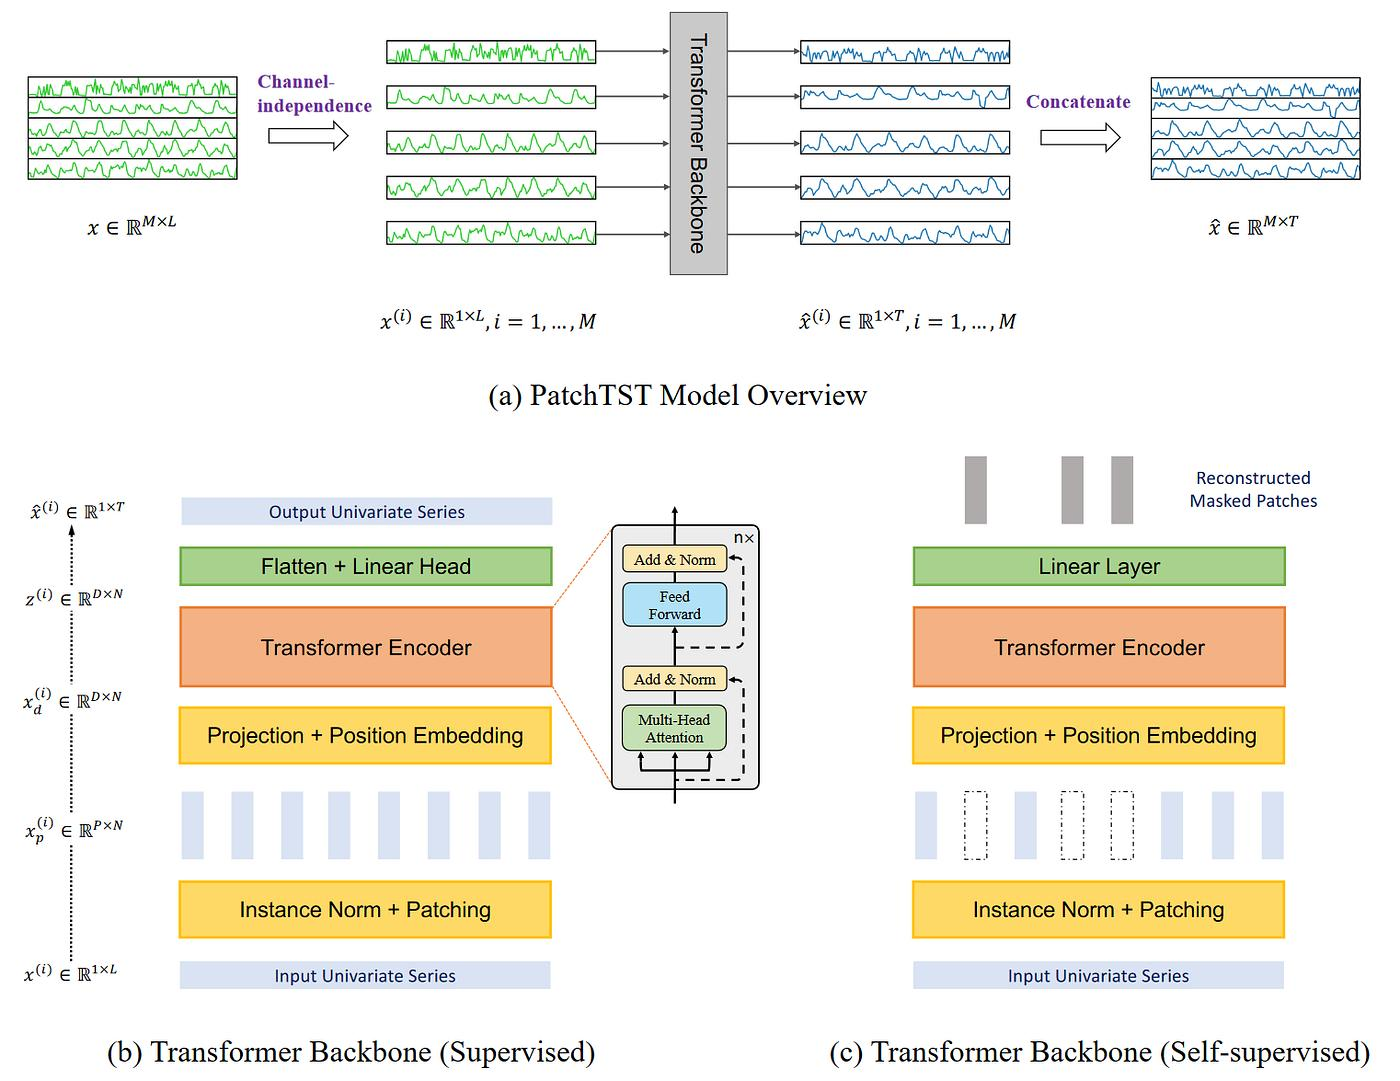
\includegraphics[width=0.60\textwidth]{patchtst_paper_figure1.jpeg}
\caption{PatchTST architecture, reproduced from Nie et al., Figure 1 \cite{nie2023patchtst}.}
\label{fig:paper_architecture}
\end{figure}
\vspace{-1.4em}

\begin{figure}[H]
\centering
\begin{minipage}{0.485\textwidth}
\centering
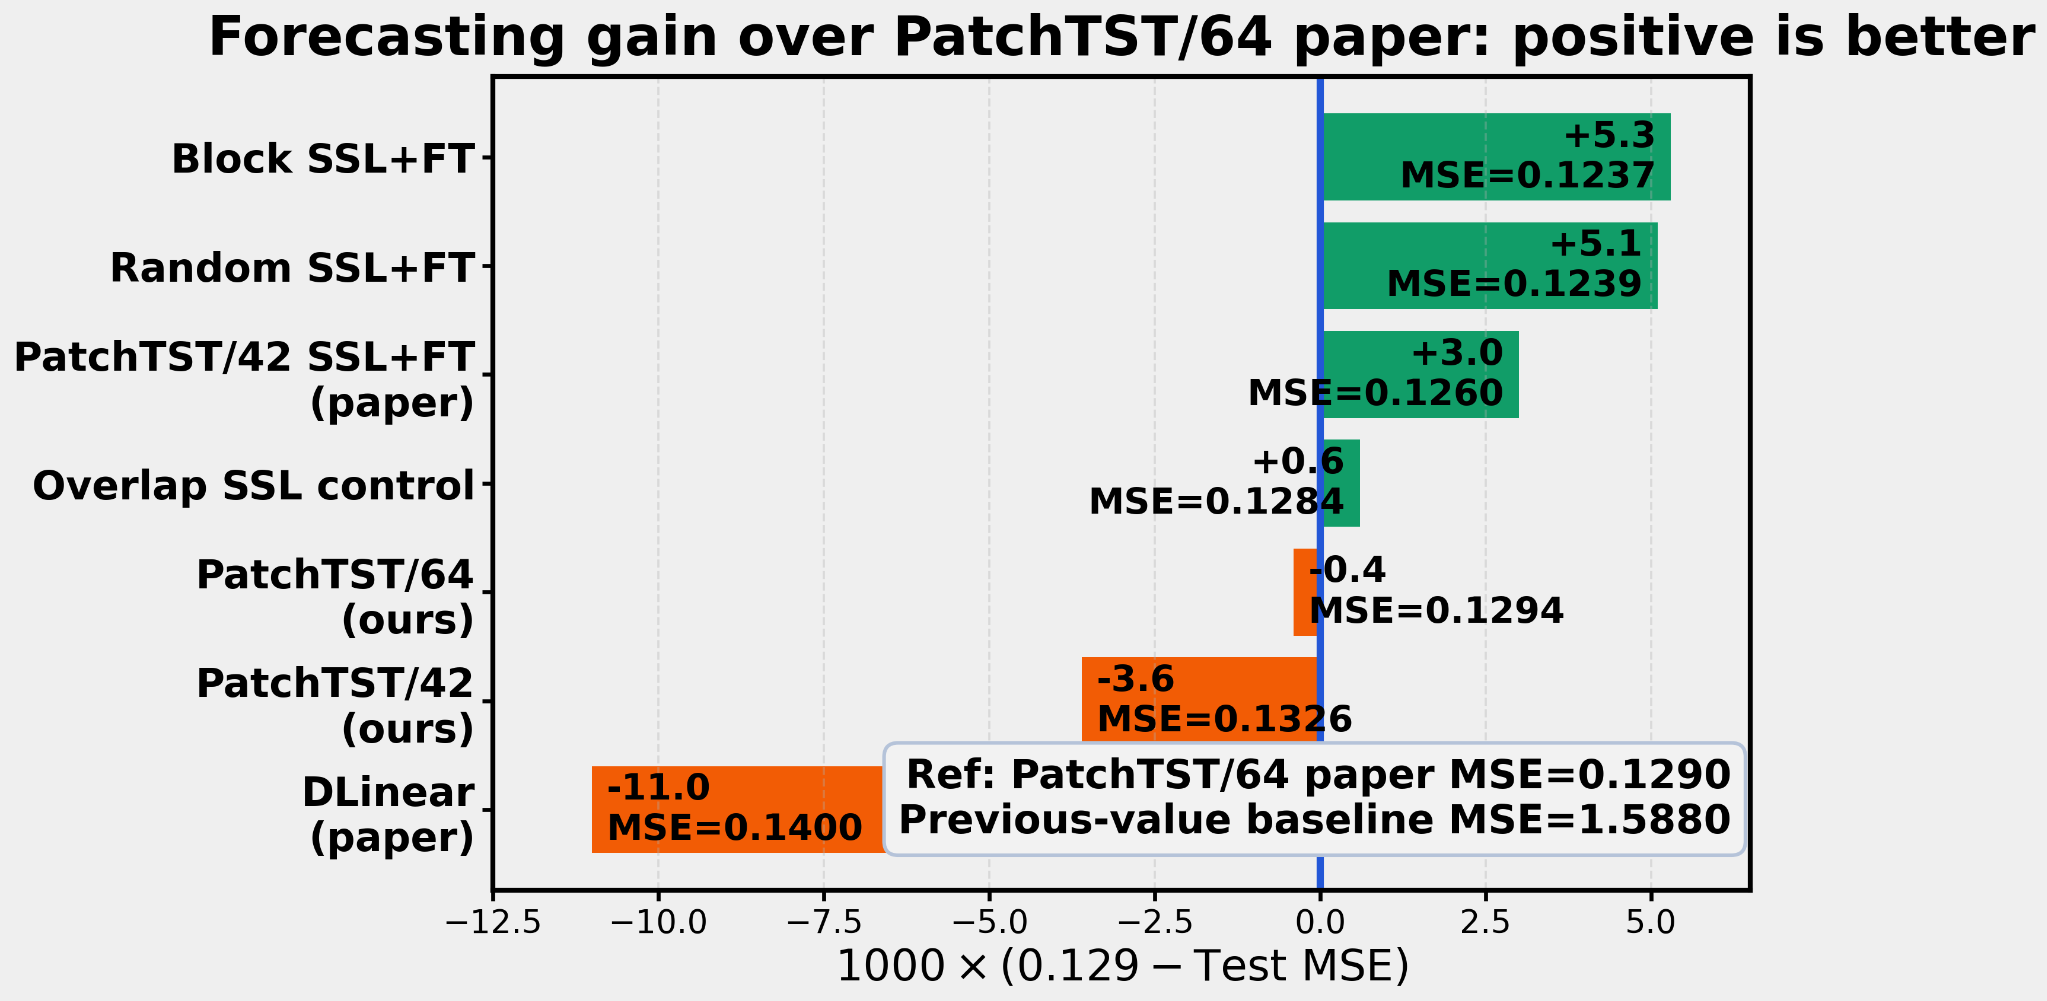
\includegraphics[width=\linewidth]{forecasting_gain_user.png}
\caption{Project result figure. Positive gain means lower MSE than the PatchTST/64 paper baseline.}
\label{fig:forecasting_gain}
\end{minipage}\hfill
\begin{minipage}{0.485\textwidth}
\centering
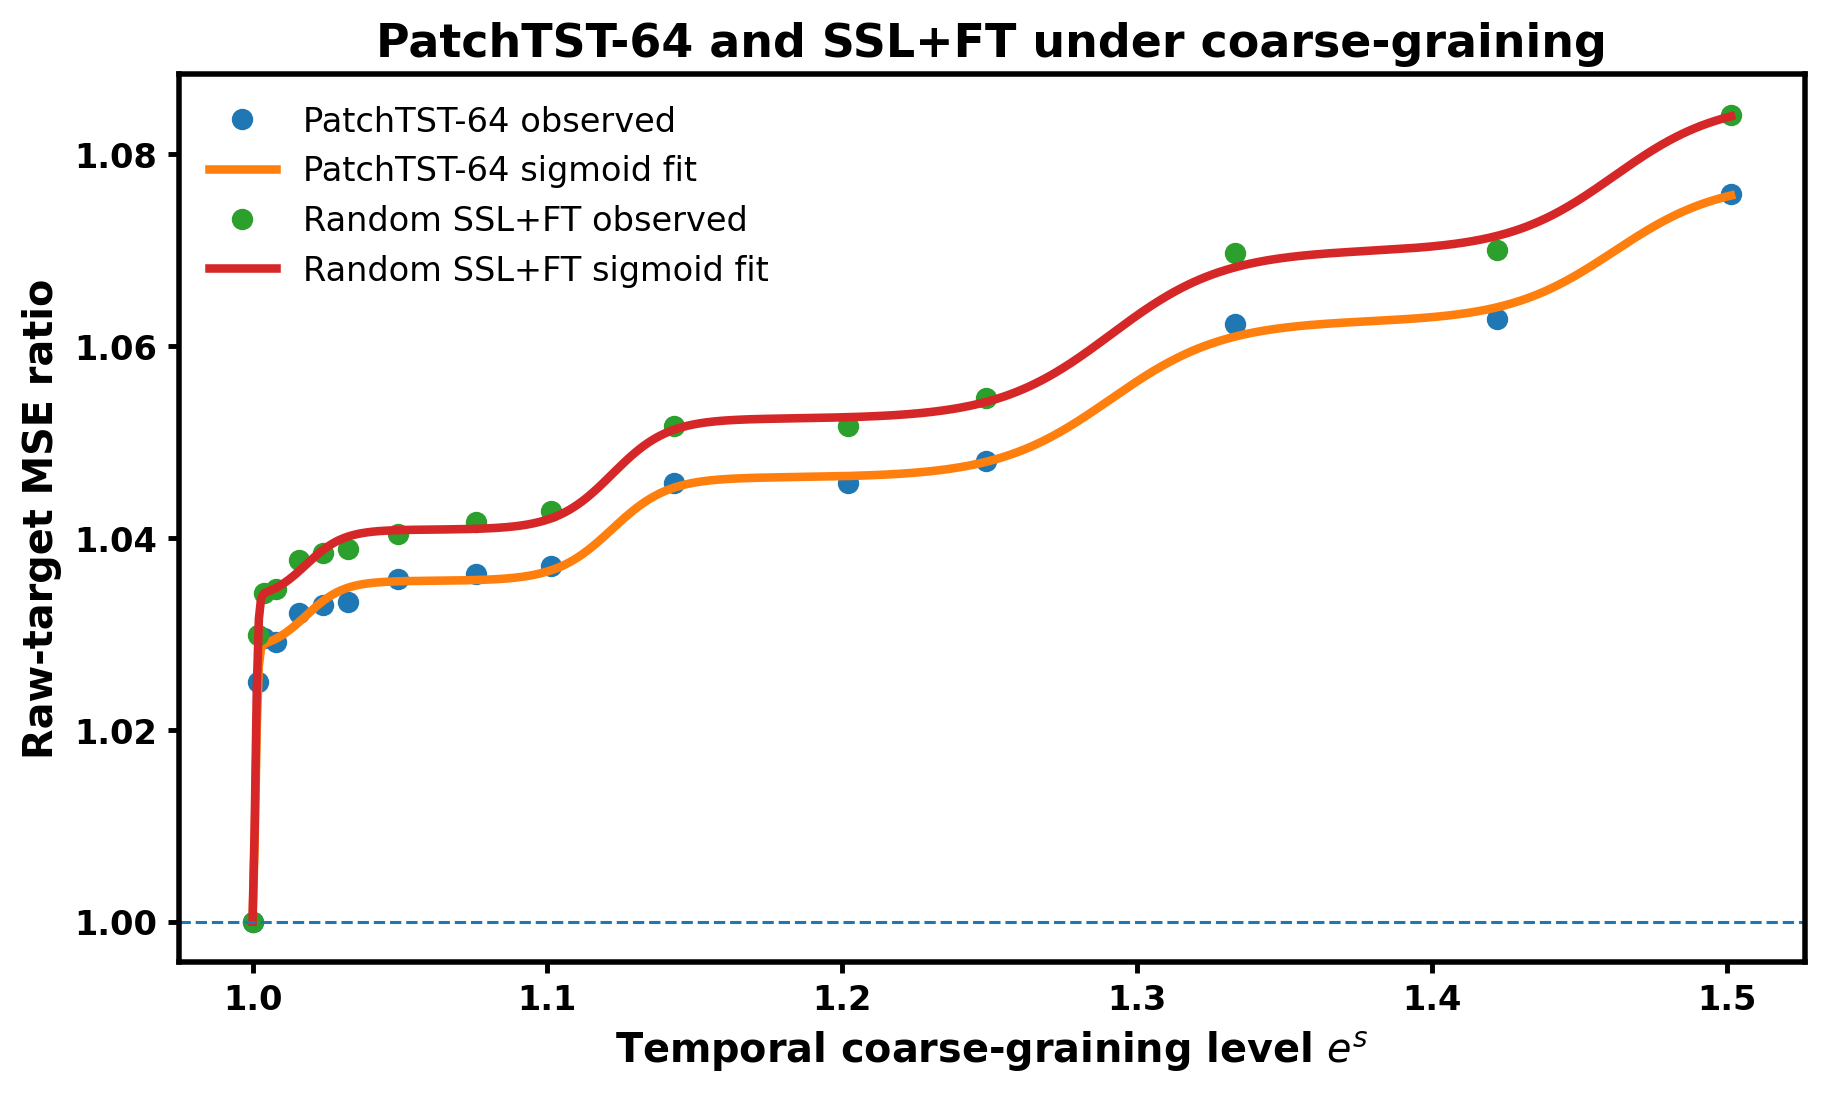
\includegraphics[width=\linewidth]{scale_sensitivity_user.png}
\caption{Scale probe. Higher raw-target MSE ratio means stronger degradation after coarse-graining.}
\label{fig:scale_sensitivity}
\end{minipage}
\end{figure}
\vspace{-1.3em}

\begin{table}[H]
\centering
\scriptsize
\caption{Complete numerical summary.}
\label{tab:complete_results}
\begin{tabular}{lcccccc}
\toprule
Method & $L$ & $H$ & $P$ & $S$ & pre/FT & Test MSE \\
\midrule
Previous-value baseline & 512 & 96 & -- & -- & 0/0 & 1.5880 \\
DLinear paper baseline & 512 & 96 & -- & -- & -- & 0.1400 \\
PatchTST/42 supervised & 336 & 96 & 16 & 8 & 0/30 & 0.1326 \\
PatchTST/64 paper reference & 512 & 96 & 16 & 8 & -- & 0.1290 \\
PatchTST/64 supervised & 512 & 96 & 16 & 8 & 0/30 & 0.1294 \\
Overlap SSL control & 336 & 96 & 16 & 8 & 30/15 & 0.1284 \\
Paper SSL fine-tuning & 512 & 96 & 12 & 12 & 100/30 & 0.1260 \\
Random SSL+FT & 512 & 96 & 12 & 12 & 30/15 & 0.1239 \\
Block SSL+FT & 512 & 96 & 12 & 12 & 30/10 & \textbf{0.1237} \\
\bottomrule
\end{tabular}
\end{table}

\end{document}
